\chapter{Verification and Validation}\label{ch:validation}

The numerical methods of the preceding chapters are exercised by an automated test suite of about
\num{2450} tests, plus \num{18} slow ones that need external data and run separately. The large majority guard low-level invariants --- array shapes, configuration parsing,
byte-for-byte reproducibility --- and are not individually informative. This chapter does not enumerate
them. Instead it describes the tests that verify the numerical \emph{physics} against independent
references, organized by the kind of evidence they provide, and names each so that a reader may locate it.
The goal of these tests, and of this chapter, is to characterize whether the engine computes what it is
specified to compute, not to assess the physical realism of any simulation. Validation suites with pinned
tolerances are themselves tested: the code or the data is perturbed on purpose in a number of ways, and each
pin must fail; where a result has a natural ordering --- a finer resolution closer to the reference --- the
ordering is pinned as well.

\section{Closed-form analytic flows}\label{sec:val-analytic}

The most direct evidence comes from flows whose trajectories are known in closed form, for which the
computed path can be compared against the exact solution. The suite includes uniform flow, helical rotation
(with a test that the orbital radius is conserved), a Burgers vortex, inertial oscillations, an Ekman spiral,
and incompressible linear strain, whose exponential trajectory is matched to $2\cdot10^{-6}$ degrees
horizontally and \SI{8}{mm} vertically. Linear strain, solid-body rotation and downwelling are repeated on
quadrilateral meshes. In each case
the particle is integrated through the analytic field and its position checked against the formula, to
tolerances far below the grid scale. The edge least-squares scheme is checked to be exact for linear fields
inside triangles and quadrilaterals, to carry a flow parallel to a wall exactly under free slip, and to give
the same result on either side of the dateline. The adaptive scheme's coefficients are checked against the
Dormand--Prince order conditions, and its accuracy on a vortex against the tolerance and against RK4.

\section{Conservation and statistics}\label{sec:val-conservation}

A second class of tests checks conserved quantities and statistical laws that the numerics must respect.
For the three-dimensional vertical advection, the key tests exploit continuity: in a steady, divergence-free
flow a streamfunction exists and must be conserved along trajectories. Integrated through an analytic
downwelling cell, particles keep the streamfunction to 0.15\,\%; through an Ekman-pumping cell, to 3\,\% over
200 steps with the default vertical combine and 5\,\% over 100 steps with every combine. These are what verify
that the vertical-velocity interpolation neither creates nor destroys volume.

For the stochastic schemes, the ensemble variance is checked to grow as $\sigma^2=2K_h t$
(\cref{ch:diffusion}). On the sphere, the Monte-Carlo mean change of $\sin\latx$ under the horizontal kicks is
checked against the generator of the spherical random walk, $-2K_y\,h\sin\latx/R_M^2$ --- the walk on the
longitude--latitude chart gives half of it --- and particles are checked to cross a pole cleanly. In the
vertical, a uniform column in a diffusivity that varies tenfold must stay uniform: after \num{5000} steps each
of eight depth bins stays within 20\,\% of its share, forward and backward; without the drift term the density
would follow $1/A_z$ instead.

\section{Contracts with model data}\label{sec:val-data}

Some properties can only be checked against real model output; these tests run when the data are available
and are skipped otherwise. The sign of the vertical velocity (\cref{sec:vert-wsign}) is tested end to end ---
a file value of $+10^{-4}$\,m/s positive upward lifts a particle \SI{8.64}{\metre} in one Euler day --- and
against physics: in the equatorial Pacific at \SI{50}{\metre} the mean vertical velocity read from native
FESOM2 output, and from its HEALPix remap, must be upward. The HEALPix remaps are validated against the native
model: the same seeds run for thirty daily RK2 steps on the native mesh and on three HEALPix resolutions, and
the tests pin the ratio of median displacements, the median separation of paired trajectories, the mean
drift, the survivors, the ordering --- the finest remap closest to the native run --- and the equality of the
time axes, which catches a uniform one-day offset that the statistics alone would miss.

The sigma step of \cref{sec:vert-sigma-step} has exact solutions: with a tide, a sloping bottom, a horizontal
flow and a uniform dia-sigma velocity, the fraction of the column is linear in time, and Euler, RK2 and RK4
reproduce it to a relative $10^{-9}$, forward and backward, with uniform and stretched sigma levels; with a
dia-sigma velocity linear in the fraction the three schemes converge at orders one, two and four.

\begin{figure}[t]
\centering
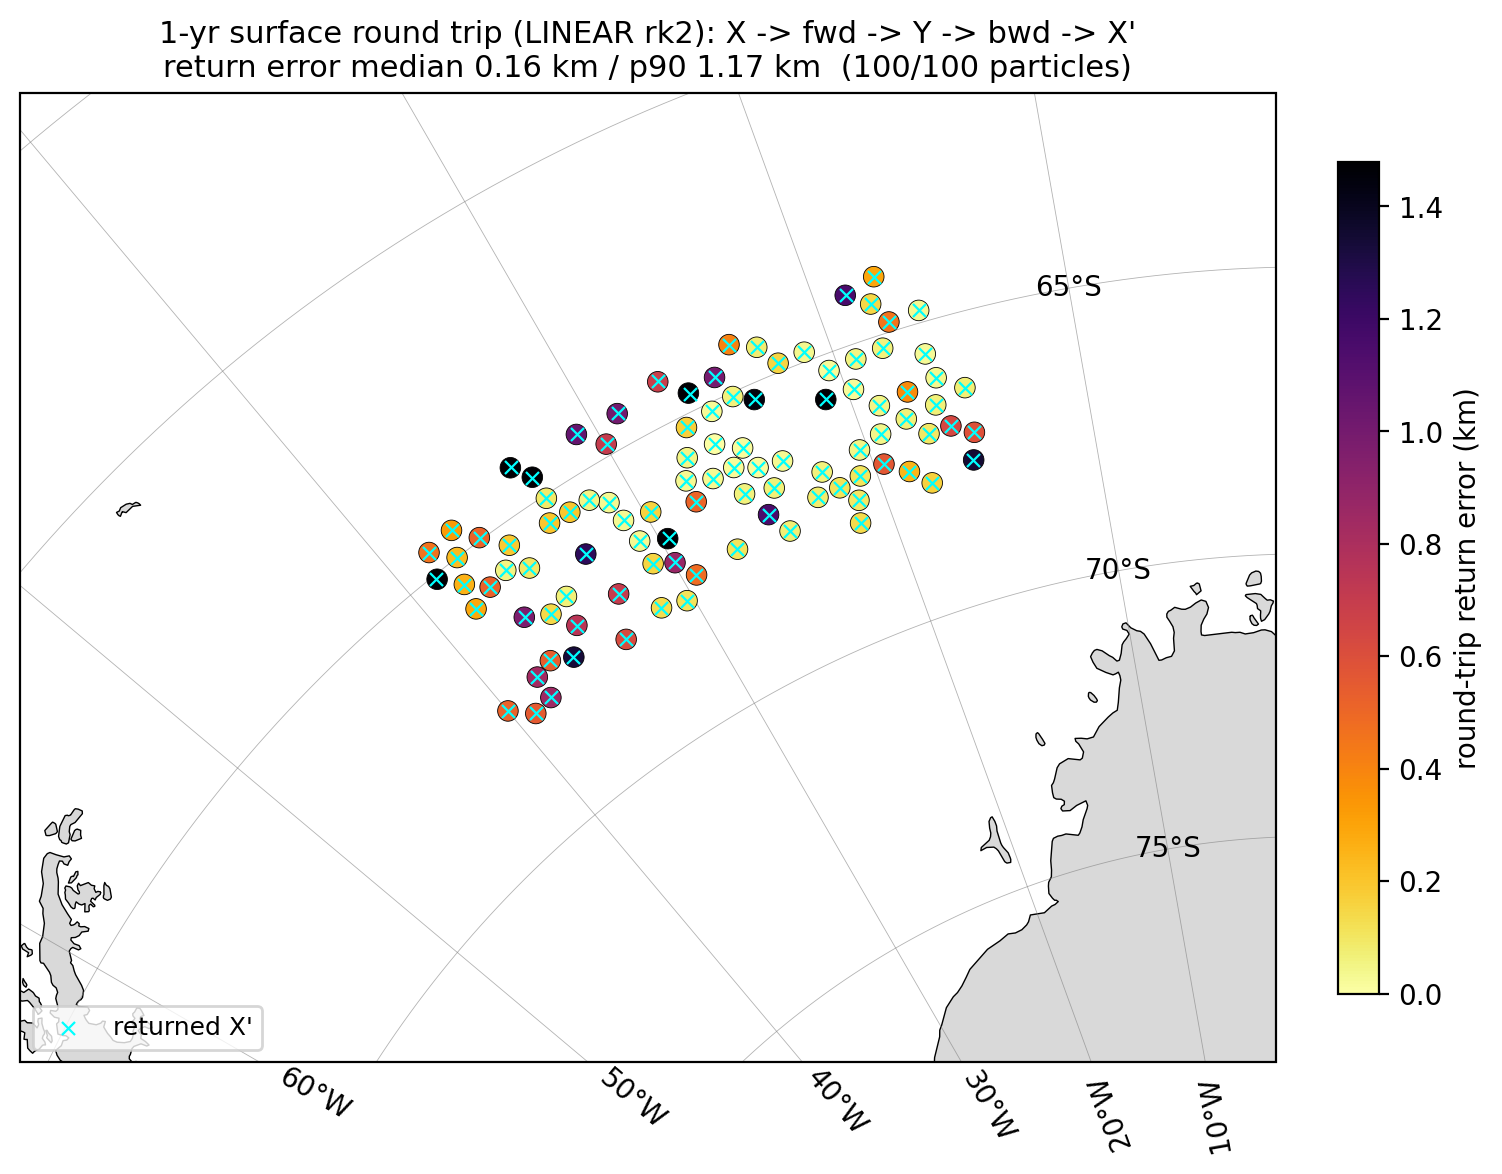
\includegraphics[width=0.72\linewidth]{revtest_roundtrip.png}
\caption{A controlled reversibility check on the \emph{core2} mesh, measured in June 2026: one hundred
particles are integrated forward for one year and then backward for one year with the same scheme (RK2,
linear reconstruction in time), and the return error between the start and end positions is mapped. The
median return error is \SI{0.16}{\kilo\metre} (ninetieth percentile \SI{1.17}{\kilo\metre}), far below the
local grid scale of tens of kilometres (a three-dimensional run at \SI{5}{\metre} depth in the Weddell Sea,
engine of June 2026; the vertical motion was negligible). Larger separations over long windows reflect Lagrangian chaos and
boundary clamping rather than a defect of the scheme.}
\label{fig:roundtrip}
\end{figure}

\section{Reversibility and determinism}\label{sec:val-reversibility}

A further class checks structural properties of the implementation. Because the deterministic integration
direction enters only as a sign on the velocity (\cref{sec:arch-direction}), a forward run followed by a
backward run should return a particle to its origin; the suite verifies this on analytic fields, including
under the monotone-cubic reconstruction, to $10^{-6}$ degrees in longitude, $10^{-9}$ in latitude and
\SI{1}{\micro\metre} in depth. The same property holds empirically on the \emph{core2} mesh: a clean one-year
surface round trip returns one hundred particles to a median of \SI{0.16}{\kilo\metre} (\cref{fig:roundtrip}).
With diffusion the backward run is the adjoint process, not the reversal of the forward one
(\cref{sec:diff-model}), and the tests check that the backward drift is kept.

Determinism is checked separately, as bit-for-bit identity. The fused and unfused kernels must agree for every
fused family, including the three-dimensional barycentric RK2 kernel and the monotone-cubic kernels
(\cref{ch:fused}); the exact nearest-node search must match a brute-force search on random geometries, and the
nearest-node kernels must match frozen copies of their earlier versions, ties included; element tracking must
give the same verdicts as the ring search. A resumed run must reproduce the uninterrupted one --- with
beaching, vertical diffusion, element tracking and sampling --- and must record the same steps; a checkpoint
interrupted mid-write must never load; a sharded release merged back must equal the unsharded run in its
data; and a run with the shared snapshot cache must equal one without it. The counter-based random numbers (\cref{sec:diff-rng}) are
independent of the thread count by construction: each draw depends only on its key.

\section{Time-dependent benchmark flows}\label{sec:val-benchmarks}

A constant zonal flow, a time-dependent moving eddy and a decaying eddy are integrated and compared with
their closed forms. A step-refinement test confirms the second-order ceiling
that linear-in-time reconstruction imposes on the whole scheme: halving the step cuts the RK4 error by a factor
between 3.5 and 5, not sixteen --- the $O(\Delta t^2)$ cap of \cref{ch:temporal} that the monotone-cubic
reconstruction lifts. Two diffusion benchmarks check the moments of Brownian motion and the skewness that a
spatially varying diffusivity must produce. These suites are marked slow and run outside the default test
run.

The engine adopts a metre-per-degree constant that differs from that of the original Fortran code, which
intentionally breaks bit-parity with it; the Fortran comparison is therefore not part of the suite, and the
Fortran prototype and its reference trajectories are not part of this repository.

\codeanchor{The physics-validation tests live in \srcfile{tests/}: the analytic-flow and streamfunction
families (\fn{test\_analytical\_3d\_benchmarks.py}, \fn{test\_downwelling\_psi.py}, \fn{test\_3d\_analytical.py},
\fn{test\_quad\_mesh\_benchmarks.py}); the random walks (\fn{test\_spherical\_random\_walk.py},
\fn{test\_az\_diffusion.py}); the data contracts (\fn{test\_w\_sign\_contract.py},
\fn{test\_healpix\_native\_twin.py}, \fn{test\_fesomc\_w\_contract.py}); the bit-identity pins
(\fn{test\_fused\_3d\_bary.py}, \fn{test\_exact\_nearest.py}, \fn{test\_node\_xyz.py}, \fn{test\_edge\_walk.py},
\fn{test\_checkpoint\_integrity.py}, \fn{test\_sharding.py}); and the reconstruction-order tests
(\fn{test\_temporal\_reconstruction.py}); the benchmark flows and diffusion benchmarks are the suites marked
slow.}
